\subsection{Geometria}

\begin{figure}
	\center
	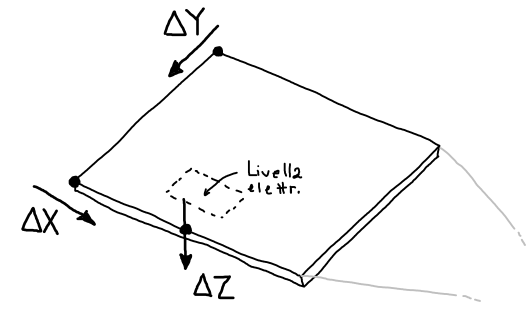
\includegraphics[width=20em]{geometriamis}
	\caption{\label{fig:geometriamis}
	Misura della geometria di una lastra di scintillatore.
	La \emph{profondità} $\Delta Z$ è misurata con il metro a nastro
	con riferimento la lastra più in alto (PM6).
	I \emph{disallineamenti} $\Delta X$ e $\Delta Y$ sono misurati
	con il righello o il metro a nastro usando come riferimento
	una livella a bolla.
	Le \emph{inclinazioni relative} $\alpha_0$ e $\beta_0$ sono misurate con
	una livella elettronica (un telefono) che ha una risoluzione di \SI{0.1}{\degree}.}
\end{figure}

\begin{table}
	\center
	\begin{tabular}{cccccccc}
		PM & $\Delta X$ [\si{mm}] & $\Delta Y$ [\si{mm}] & $\Delta Z$ [\si{mm}] & $\alpha_0$ [\si\degree] & $\beta_0$ [\si\degree] & $L_x$ [mm]      & $L_y$ [mm]      \\
		\hline
		6  & 0                    & \num{543 \pm 1}      & 0                    & 0.7                     & 0.2                    & \num{400 \pm 2} & \num{482 \pm 1} \\
		5  & \num{-5 \pm 1}       & \num{540 \pm 1}      & \num{102 \pm 1}      & 1.0                     & 0.3                    & \num{404 \pm 2} & \num{482 \pm 1} \\
		4  & \num{1 \pm 1}        & \num{536 \pm 1}      & \num{205 \pm 1}      & 1.2                     & 0.4                    & \num{398 \pm 2} & \num{481 \pm 1} \\
		3  & \num{1 \pm 1.4}      & \num{539 \pm 1}      & \num{308 \pm 1}      & 0.8                     & 0.3                    & \num{400 \pm 2} & \num{480 \pm 1} \\
		2  & \num{2 \pm 1.4}      & \num{531 \pm 1}      & \num{411 \pm 1}      & 0.2                     & 0.6                    & \num{395 \pm 2} & \num{481 \pm 1} \\
		1  & \num{0 \pm 2}        & non mis.             & \num{804 \pm 2}      & 0.8                     & 0.4                    & \num{398 \pm 2} & \num{480 \pm 1}
	\end{tabular}
	\caption{\label{tab:geom}
	Misure di geometria.
	Per gli angoli abbiamo preso un'incertezza pari a metà della risoluzione cioè \SI{0.05}\degree.
	Le incertezze delle misure con righello o metro a nastro
	le abbiamo fissate a una tacca o a due tacche
	a seconda della difficoltà della misura.
	Le misure con incertezza \num{1.4} sono ottenute
	sommando due misure con incertezza \num{1}.
	Per il $\Delta Y$ non misurato,
	prendiamo la media degli altri $\Delta Y$ come valore nominale
	e la deviazione standard campione come incertezza.}
\end{table}

Dobbiamo misurare le caratteristiche geometriche dell'apparato
per assegnare misure alle variabili del modello in \autoref{fig:geometriadef}.

Con una livella a bolla controlliamo che tutte le lastre siano orizzontali.
La livella a bolla ha, per verifica empirica, una risoluzione minore di quella
elettronica del telefono (\SI{0.1}{\degree}).
Tuttavia la livella elettronica non ha uno zero fisso; lo zero va impostato
appoggiandola su una superficie di riferimento.
Allora misuriamo l'inclinazione delle lastre con la livella elettronica 
(gli angoli di Eulero del telefono forniti dal software, che chiamiamo $\alpha_0$ e $\beta_0$),
\marginpar{Controllare con il telefono di Bob se sono effettivamente questi angoli
come li sto definendo fin'ora.}
e poi assumiamo, come detto nella \autoref{sec:teogeom},
che l'inclinazione media delle lastre sia nulla.
Questo ci permette di valutare in modo quantitativo quantomeno l'incertezza
dovuta all'inclinazione relativa delle lastre.

Misuriamo la posizione spaziale usando righello, metro a nastro e livella a bolla.
Facendo riferimento alla \autoref{fig:geometriamis} per la notazione, riportiamo
in \autoref{tab:geom} le misure.
\marginpar{Aggiungere come si passa dalle misure alle variabili del modello e l'incertezza del calcolo
(incertezza Monte Carlo, incertezza dovuta alle misure).}

Riportiamo le formule per passare dalle misure al modello.
Per convertire le inclinazioni relative in assolute,
sapendo che gli angoli sono piccoli facciamo direttamente la media sugli angoli:
\begin{align*}
	\alpha &= \alpha_0 - \langle\alpha_0\rangle, \\
	\beta  &= \beta_0  - \langle\beta_0\rangle.
\end{align*}
I parametri di una lastra (equazione \ref{eq:lastra}) sono dati da
\begin{align*}
	\hat V_x &= \begin{pmatrix}
		\cos\alpha, & 0, & \sin\alpha
	\end{pmatrix} \\
	\hat V_y &= \begin{pmatrix}
		\sin\alpha\sin\beta, & \cos\beta, & -\cos\alpha\sin\beta
	\end{pmatrix} \\
	\vec P &= \begin{pmatrix}
		\Delta X, & \Delta Y - L_y\hat V_y\hat y, & -\Delta Z - \frac12 L_x\hat V_x\hat z
	\end{pmatrix}.
\end{align*}
